\subsection{Version control system}

\subsubsection{Tortoise SVN}

TortoiseSVN is free, open-source revision control/version control/source control software for Windows. It is a standalone Apache Subversion client which is not integrated with specific IDE, so it can be used with any development tools.\newline

Since it is based on subversions, TortoiseSVN has all the features of subversion. It supports mors current CVS (Concurrent Versions System) features, directories, renaming, file meta-data etc. Commits in this version control system are truly atomic, and there are also branching and tagging operations and efficient handling of binary files. \newline

\subsubsection{GitHub}

GitHub is a web-based hosting service for software development projects that use the Git revision control system. GitHub offers both commercial plans and free accounts for open source projects.\newline

Collaboration on Github is not complicated but also not intuitively clear for beginners because not all parts of the workflow are incorporated into the Github user interface. This description describes the structure of collaboration between the contributors and the maintainers of a project that is hosted on github. For every step in the workflow the respective git commands are given for reference.\newline

\begin{figure}[htb]
	\centering
	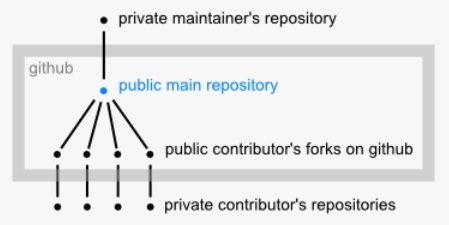
\includegraphics[width=0.6\textwidth]{prestudy/github.jpg}
	\caption{Distributed setup of git repositories}
	\label{fig:github}
\end{figure}

\newpage
